\section{System Model and Formalization\label{system_model}}

\subsection{Component Architecture}

Components are the basis of any re-usable concurrent software systems.
We adopt Szyperski's definition of components~\cite{component_software}:
\begin{quote}
  A software component is a unit of composition with contractually specified interfaces and explicit context dependencies only.
  A software component can be deployed independently and is subject to composition by third parties. 
\end{quote}
A component architecture defines components and how they execute and interact.
For example, a component in a multi-threaded component architecture consists of private state that is accessed through synchronous function call.
Components can be configured to use one another and can execute concurrently.
This section outlines a component model and architecture for an event-based system.

\paragraph{Components.}
A \emph{component} consists of state variables and a set of event handlers.
Each event handler is only allowed to modify the state of the component to which it belongs.
The absence of shared state ensures that each component can be deployed independently.
Event handlers can either be an \emph{output} that produces a signal or value, an \emph{input} that consumes a signal or value, or an \emph{internal} that neither produces nor consumes a signal or value.
Components can be created and destroyed at run-time.

\paragraph{Binding.}
A \emph{binding} is an association between an output and an input.
An output can be \emph{bound} to zero or more inputs subject to type compatibility.
An input can be bound at most once.
Outputs and inputs can either be \emph{public}, available for binding by external components, or \emph{private}, only available for binding by the containing component.
Internals are always private.
Events can be bound and unbound at run-time.
The component requesting that an output be bound to and input is said to be the \emph{owner} of the binding.
Private outputs and inputs can only be bound by the containing component.

\paragraph{Execution.}
Execution proceeds by randomly selecting and atomically executing outputs and internals.
When an output is executed, both the output all bound inputs are executed in one atomic step receiving the value produced by the output if applicable.
Two events can be executed concurrently if the set of components implied by each event are disjoint.
All components have outputs for creating, binding, unbinding, and destroying and inputs for receive results that are permanently bound to ``the system.''
System calls follow a request-reply system where a component sends a request for a create, bind, unbind, or destroy, the system receives the request, the system processes the request, the system sends a reply, and the component receives the reply.

\paragraph{Composition.}
Binding, atomic execution, and the absence of shared state allows components to be composed, i.e., combined in such a way as to yield a valid component.
Components can be composed by 1) concatenating their state variables, 2) renaming events so every event's name is unique, and 3) folding input events into the output events to which they are bound.
Composition allows the programmer to reason about a constellation of components as a single component.
Often, the properties of the resulting component can be reasoned about using the properties of the constituent components.
Components can be composed at compile time using the process outlined above, however, it is often better to preserve component boundaries to take advantage of concurrent execution.

\begin{figure}
\center
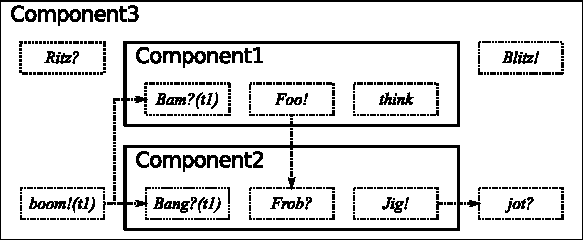
\includegraphics{system_model}
\caption{Example composable event-based system.
  Components are depicted as solid rectangles, e.g., Component3.
  Events (outputs, inputs, and internals) are depicted as dotted rectangles, e.g., \emph{Ritz?}.
  Output events are suffixed with \emph{!}.
  Inputs are suffixed with \emph{?}.
  Internals have no suffix.
  Public events start with an uppercase letter.
  Private events start with a lowercase letter.
  Bindings are indicate by dotted lines with an arrow pointing to the input.}
\label{sys_model}
\end{figure}

\paragraph{Example.}
Figure~\ref{sys_model} depicts a fictitious system of three components.
Component3 contains a public input \emph{Ritz?} and a public output \emph{Blitz!}.
Component3 also contains a private output \emph{boom!(t1)} that produces a value of type \emph{t1} and a private input \emph{jot?}.
Component3 contains two components: Component1 and Component2.
Component1 contains a public input \emph{Bam?(t1)}, a public output \emph{Foo!}, and a private internal \emph{think}.
Component2 contains a public input \emph{Bang?(t1)}, a public input \emph{Frob?}, and public output \emph{Jig!}.
All bindings are owned by Component3.
The output \emph{boom!(t1)} is bound to inputs \emph{Bam?(t1)} and \emph{Bang?(t1)} and shows how one output can be bound to multiple inputs.
The output \emph{Foo!} is bound to input \emph{Frob?} and shows how an output in one component can be bound to input in another component by a third component.

Opportunities for concurrent execution exist for the system depicted in figure~\ref{sys_model}.
The set of components implied by \emph{Blitz!} is \{Component3\} while the set of components implied by \emph{Foo!} is \{Component1, Component2\}.
Since the sets are disjoint, \emph{Blitz!} and \emph{Foo!} can be executed concurrently.
The set of components implied by \emph{boom!(t1)} is \{Component1, Component2, Component3\}.
Consequently, \emph{boom!(t1)} cannot be executed concurrently with any other event.

%% \subsection{Requirements}

%% Our system model is motivated by the semantics of devices, the semantics of distributed systems, and the desire for conceptual integrity.
%% We adopt a recursive view that nodes, i.e., devices, in a distributed system may themselves be represented as a distributed system consisting of different sensors, actuators, and processes.
%% We use the term \emph{node} to refer to a participant in a typical distributed system, i.e., one that uses standard network links.
%% We use term \emph{module} to refer to a computational element within a node.
%% Modules that reside on the same node are said to be \emph{collocated}.

%% \paragraph{Local State.}
%% We require that all modules and by extension all nodes only manipulate local state.
%% Said another way, there is no global or shared state.
%% Computation designed around the manipulation of local state only is easily modularized and consequently, easier to distribute and execute concurrently.

%% \paragraph{Message Passing.}
%% Nodes in distributed systems interact by passing messages over communication links.
%% Message passing can either be synchronous or asynchronous.
%% In synchronous message passing, the events of message production and delivery are the same, i.e., atomic.
%% In asynchronous message passing, the events of message production and delivery are logically distinct events subject to being interposed by other events.
%% Synchronous message passing is most often used between modules on the same node while asynchronous message passing is most often used between nodes.
%% Both synchronous and asynchronous message passing are required.
%% Synchronous message passing is necessary for building composable systems because of it association with atomicity.
%% Asynchronous message passing is necessary for building real distributed systems as this matches the semantics of the networks found in practice.

%% \paragraph{Asynchronous Atomic Events.}
%% Events are natural way to deal with the asynchrony involved in receiving messages from the network or interacting with the physical environment.
%% This implies that the model contains a general treatment of events, i.e., modules can both produce and consume events.
%% Modules, therefore, are reactive and structured as a set of atomic event produces and consumers.
%% The guarantee of atomicity obviates the need for concurrency control primitives and improves our ability to reason about the behavior of the module.
%% Modules communicate using events according to a \emph{configuration} that determines which events are delivered to each module.

%% Communicating with external resources such as the operating system or physical environment is foundational to writing useful programs.
%% Consider the history of I/O in the C run-time library.
%% The synchronous function call semantics of the C programming language made it possible to write system calls, e.g., read and write, that transfer control to the operating system which then completes the operation and return control to the process after the system call.
%% This is called \emph{blocking I/O} because the process blocks while it waits for the operating system to complete the I/O.
%% Blocking I/O has the severe restriction that only one I/O source can be used at a time.
%% To remedy this, system calls such as select and poll were introduced that allow a process to monitor I/O sources for events and then respond to these events.
%% Asynchronous I/O was a further advancement that allows for the system (instead of the process) to dispatch a function upon the completion of I/O.
%% Compare this to UNIX signals that are neither general (fixed-number with no associated data) nor principled.
%% Interrupts are difficult to use correctly.

%% \paragraph{Dynamics.}
%% The set of nodes and communication links is dynamic in real distributed systems.
%% Similarly, the set of modules and their configuration in real devices can change as the device may be re-purposed by users over time.
%% In general, our system model must support a dynamic number of modules and, consequently, dynamic configuration of those modules.

%% \paragraph{Reflection.}
%% The ability to dynamically configure a module implies that a module must be able to know its configuration status to preserve certain properties.
%% For example, consider a module for a reliable FIFO queue.
%% Since the queue can be dynamically configured, the queue must be able to determine if the event produced by removing and returning an item from the queue will be delivered.
%% Otherwise, the queue will lose data items and therefore not be reliable.

\subsection{I/O Automata}

The Input/Output (I/O) automata model was developed by Lynch~\cite{distributed_algorithms} to model reactive concurrent and asynchronous systems.
An I/O automaton consists of state variables and atomic actions that manipulate the state.
The three action types are inputs, outputs, and internal actions.
Input actions receive a signal or a value and output actions produce a signal or a value.
Internal actions just manipulate the state of the automaton.
Output and internal actions are \emph{locally controlled actions}~\cite{distributed_algorithms} are often presented as precondition and an effect.
Input and output actions are \emph{external actions}~\cite{distributed_algorithms} because they allow an automaton to communicate with other automata.
Automata may \emph{composed} by concatenating the state variables of the constituent automata and incorporating the effects of input actions into output actions with the same name.
A useful operation in composite automata is \emph{hiding} which converts an output action to an internal action.
Composing automata results in a static configuration, i.e., the set of automata and their interactions are fixed.
Execution in the I/O automata model consists of repeatedly selecting a local action and then applying the effect if the precondition is true.
The scheduler is assumed to be fair meaning that a local action is guaranteed to be selected (but not executed) infinitely often.

The proposed system has a straightforward mapping to the I/O automata model: components are automata and events are actions.
However, the I/O automata model assumes a static configuration while the proposed system requires the ability to deal with dynamic configurations, i.e., creating, binding, unbinding, and destroying.

\subsection{I/O Automata and Dynamic Configuration}

A standard technique for modeling dynamic modules in I/O automata is to assume they exist but are inactive.
Dynamic automata can then be activated and deactivated using inputs.
We will use a similar technique to model dynamic configurations.

We introduce a \emph{system automaton} that records the configuration of all automata in the system.
We differentiate between automaton types and automaton instances.
Every automaton instances has a unique \emph{automaton identifier (aid)}.
The state of the system automaton consists of the set of aids $A$ indicating what automata exist and a set of binding records $B$ indicating the relationship between output and input actions.
A binding record $(out, output, in, input)$ is tuple consisting of the aid of the output automaton $out$, the name of the output action $output$, the aid of the input automaton $in$, and the name of the input action $input$.

The configuration contained in set of binding records must be a valid static configuration to ensure that the behavior of the complete system remains analyzable under the I/O automata model.
First, the output automaton and input automaton must exist $\forall (out, output, in, input) \in B: out \in A \land in \in A$.
% TODO:  Binding must not exist.
Second, an input can only be bound to one output.
Thus, a given $in$ and $input$ combination can appear at most once in $B$.
Third, an output cannot be bound to an input in the same automaton.
Thus, $out \neq in$ for every $(out, output, in, input)$ in $B$.
Fourth, an output cannot be bound to two inputs in the same automaton.
Thus, $in_1 \neq in_2$ for all $(out, output, in_1, input_1), (out, output, in_2, input_2)$ in $B$.

The system automaton contains input actions for creating an automaton, binding an output to an input, unbinding an output and an input, and destroying an automaton and output actions that indicate the result of a create, bind, unbind, or destroy.
All automata are composed with the system automaton and contain outputs for creating, binding, unbinding, and destroying and inputs for receiving results.
Systems calls (create, bind, unbind, destroy) resemble a request-response protocol where an automaton sends a request, the system automaton receives the request, the system processes the request, the system automaton then sends the result, and the automaton receives the result.
This has the important consequence that \emph{configuration is asynchronous}.
Destroying an automaton has the effect of removing all of its bindings.
An automaton that destroys itself can therefore cause the system to deliver unbound and destroyed events without an unbind or destroy.

Using the system automaton as a bookkeeping mechanism, we can relate a statically composed system to a dynamically configured one.
The key idea is to show that actions belong to automaton $a$ are only executed when $a \in A$ and that an output action is only executed when $B$ contains all of bindings associated with the static configuration.






\subsection{Extending I/O Automata for Reflection}

Automata are endowed with additional inputs driven by system outputs indicating when an action has been bound and unbound.
Automata might use the bound input to enable processing, i.e., someone is listening so I'll start producing data.
The unbound input is useful for cleaning data structures and inhibiting further processing, i.e., no one is listening so I'll stop producing data.
The bound and unbound inputs are useful but they are also asynchronous, thus, an automaton cannot trust the status reported by the last bound or unbound for use in, for example, a precondition.

The asynchronous nature of bound and unbound requires a primitive that can examine the contents of $B$ instantaneously.
Thus, we make one exception to the rule of local state that says automata can examine the contents of $B$ to determine their current configuration.
This is permissible so long as concurrent implementations provide multiple-reader/single-writer semantics to $B$.

\subsection{Equivalence}

Extending the I/O automata model for dynamics and reflection is useless unless we can relate the extensions back to the original model or establish equivalence.
To do this, we will take advantage of the fair traces (?) property of I/O automata~\cite{distributed_algorithms}.
%% We accept an execution trace in the dynamic setting if it is a fair trace of the static model.

%% Modeling a system with I/O automata implies a fixed set of automata given by $A_0$ and set of binding records $B_0$.

Start with a trace of dynamic $T_d$.
Remove system actions from $T_d$ so $T_d'$.
We accept $T_d'$ if it is a fair trace of the static model.

Let $A_0$ be the set of automata and $B_0$ be the set of binding records in the static model.
If you want to prove correspondence, you must prove that eventually $A = A_0$ and $B = B_0$.
We also need to show that no output is executed before it is fully bound.

%% supports the actions of creating an automaton, binding an output to an input, unbinding an output and an input, and destroying an automaton.
%% Upon creation, All automata are bound
%% The four operations necessary for dynamic configuration are \emph{create}, \emph{bind}, \emph{unbind}, and \emph{destroy}.

%% \begin{outline}
%% \item State
%%   \begin{outline}
%%   \item There is no shared state in a 
%%   \item Local state only
%%   \item Shared state
%%     \begin{outline}
%%       \item Impossible in distributed systems
%%       \item Dangerous in local systems
%%     \end{outline}
%%   \end{outline}
%% \item Communication
%%   \begin{outline}
%%   \item Atomic asynchronous message passing
%%   \item Network sets size of atom (UDP)
%%   \item Can build reliable streams (TCP)
%%   \item Local equivalent is passing a value
%%   \item Model should lend itself to writing protocols
%%   \end{outline}
%% \item Asynchrony
%%   \begin{outline}
%%     \item Model must have natural support for asynchrony, i.e., event-based
%%     \item Leads to a more efficient implementation because changed state and enabled actions become obvious
%%   \end{outline}
%% \item Concurrency
%%   \begin{outline}
%%     \item Reason about systems using non-deterministic interleaving of atomic actions
%%     \item Model should admit implementations that execute concurrently
%%   \end{outline}
%% \item Dynamics
%%   \begin{outline}
%%     \item Configuration - Edges in graph of communicating components can change at run-time.
%%       \begin{outline}
%%       \item Already required in distributed settings
%%       \item Not addressed in formal models
%%       \end{outline}
%%     \item Extension - Nodes in graph of communicating components can change at run-time.
%%   \end{outline}
%%   \item Reflection
%% \end{outline}

%% I/O Automata
%% \begin{itemize}
%%   \item Compare with UNITY
%%   \item Compare with esterel
%%   \item Compare with pi calculus
%%   \item Compare with Ptolemy
%% \end{itemize}
